\chapter{Les Transistors}

%\section{Chapter Overview}
Un transistor est un dispositif à semi-conducteur utilisé pour amplifier ou commuter des signaux électriques et de puissance. C'est un composant avec (au moins) trois terminaux. Une tension ou un courant appliqué à l'un des terminaux contrôle le courant à travers une autre paire de terminaux. Comme la puissance contrôlée (sortie) peut être supérieure à la puissance de contrôle (entrée), un transistor peut amplifier un signal.\\
%We will discuss the bipolar junction transistor (BJT) and two transistors based on the field-effect, namely the junction FET and the Metal-Oxide-Semiconductor Field Effect transistor (MOSFET).
Nous discuterons des deux transistors les plus courants : le transistor bipolaire à jonction (BJT) et le transistor à effet de champ à semiconducteur métal-oxyde (MOSFET).

\section{Transistor bipolaire à jonction}
\label{sec:bipolar_junction}
Un transistor bipolaire à jonction (BJT) est formé en plaçant un semi-conducteur de type n entre deux semi-conducteurs de type p (pnp) - ou vice versa (npn), comme le montre la figure \ref{fig:bjt1}. Dans le cas du transistor pnp, la région fortement dopée $p^+$ est appelée l'\emph{émetteur} (E). La région $n$ centrale étroite est la \emph{base} (B). Sa largeur est petite par rapport à la longueur de diffusion des porteurs minoritaires. La région $p$ légèrement dopée est le \emph{collecteur} (C). La figure \ref{fig:bjt1} montre également les symboles de circuit pour les deux transistors BJT, ainsi que les directions conventionnelles pour les tensions et les courants.\
Nous discuterons en détail du transistor pnp ; le raisonnement pour le transistor npn est similaire et sera laissé en exercice.

\begin{figure}[h!]
\centering
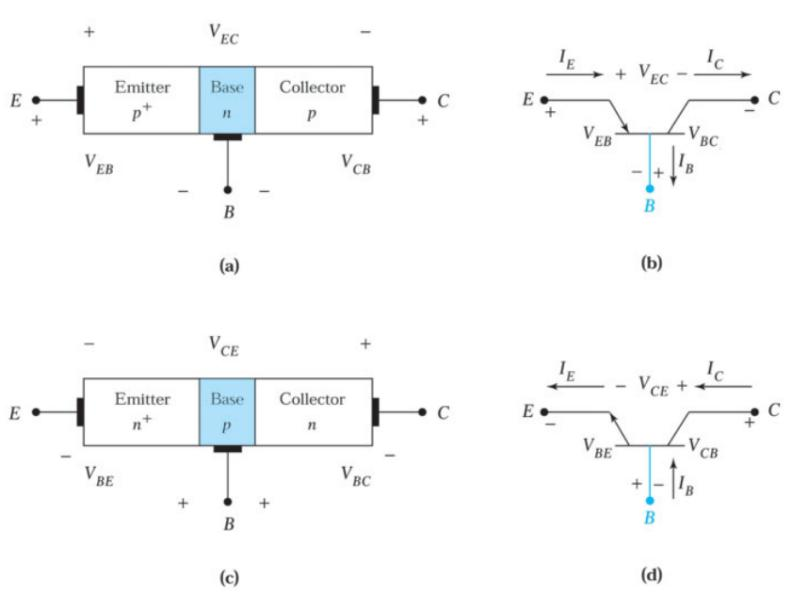
\includegraphics[width=12cm]{figures/ch01/bjt1.jpg}
\caption{(a) Schéma idéalisé unidimensionnel d'un transistor bipolaire p-n-p et (b) son symbole de circuit. (c) Schéma idéalisé unidimensionnel d'un transistor bipolaire n-p-n et (d) son symbole de circuit.} 
\label{fig:bjt1}
\end{figure}

\subsection{Fonctionnement en mode actif}
Considérons d'abord le transistor pnp avec les trois bornes (émetteur, base et collecteur) connectées à la masse comme le montre la figure \ref{fig:bjt2} (a). Dans ces circonstances, nous pouvons construire le profil de charge comme nous l'avons fait pour la jonction pn. Remarquez que les régions de charge d'espace aux deux jonctions s'étendent plus profondément dans les régions moins dopées (base dans la jonction E-B, collecteur dans la jonction B-C).

\begin{figure}[h!]
\centering
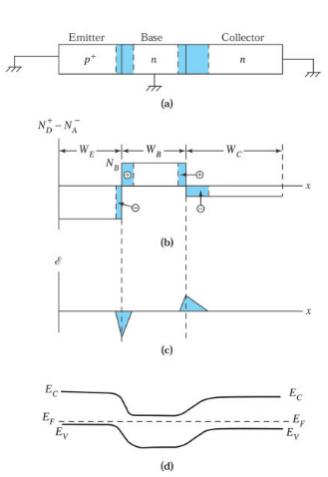
\includegraphics[width=8cm]{figures/ch01/bjt2.jpg}
\caption{(a) pnp transistor with all leads grounded (b) Charge profile in equilibrium (c) Electric field (d) Energy band diagram.} 
\label{fig:bjt2}
\end{figure}
Comme pour la jonction pn, le champ électrique qui apparaît dans la région de charge d'espace est tel qu'il est en équilibre avec le courant de diffusion dû aux gradients de concentration aux jonctions. La figure \ref{fig:bjt2}(d) montre le diagramme de bande en équilibre. Étant donné qu'il n'y a pas de courant, le niveau de Fermi $E_F$ est constant dans les trois régions.\
Nous allons polariser le transistor en mode actif. C'est le mode le plus couramment utilisé en pratique. Nous le faisons en appliquant une tension positive $V_{EB} > 0$ entre l'émetteur et la base, et une tension négative $V_{CB} < 0$ entre le collecteur et la base. La jonction pn entre l'émetteur et la base est ainsi polarisée directement, tandis que la jonction entre le collecteur et la base est polarisée en inverse.\
Puisque nous appliquons une tension positive à l'émetteur et une tension négative au collecteur (tout en gardant la base à la masse ; ceci est une configuration \emph{base commune}), nous abaissons les bandes d'énergie dans l'émetteur et les élevons dans le collecteur (tout comme dans la jonction pn) - voir la figure \ref{fig:bjt3}(d). Par conséquent, la barrière de potentiel entre l'émetteur et la base est abaissée, de sorte que les porteurs majoritaires du côté émetteur (c'est-à-dire les trous) peuvent diffuser à travers la région de charge d'espace jusqu'à la base. Si la base était beaucoup plus grande que la longueur de diffusion, presque tous les trous injectés se recombineraient avec des électrons dans la base et généreraient un courant de base, tout comme dans une jonction pn ordinaire. Cependant, comme la base est petite, la plupart des trous injectés ne se recombinent pas mais diffusent dans la région de charge d'espace entre la base et le collecteur. Là, ils sont balayés par le champ électrique vers le collecteur. En conséquence, la plupart des trous quittant l'émetteur se retrouvent dans le collecteur. Ce phénomène est appelé \emph{action du transistor}. Il est important de réaliser que le courant de collecteur dépend du courant d'émetteur et donc de la hauteur de la barrière émetteur-base et de $V_{EB}$, mais pas de la tension base-collecteur $V_{CB}$ (tant que la jonction base-collecteur est polarisée en inverse).

\begin{figure}[h!]
\centering
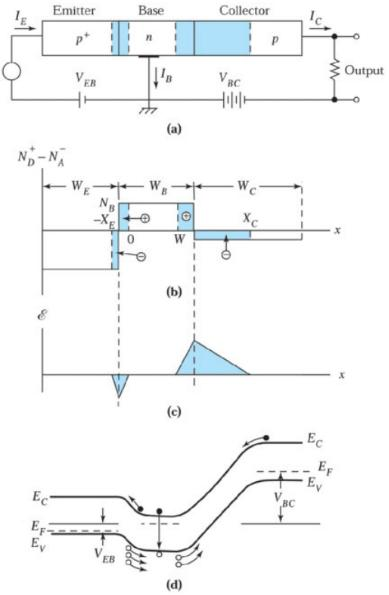
\includegraphics[width=8cm]{figures/ch01/bjt3.jpg}
\caption{pnp transistor in active mode} 
\label{fig:bjt3}
\end{figure}

\subsection{Courants en mode actif}
Pour chaque terminal, nous pouvons identifier les flux de porteurs qui contribuent aux courants $I_E$, $I_C$ et $I_B$.
\begin{enumerate}
	\item À l'émetteur :
	\begin{itemize}
		\item un courant de trous de l'émetteur vers la base $I_{Ep}$
		\item un flux d'électrons de la base vers l'émetteur $I_{En}$
	\end{itemize}
	Ainsi, $I_E = I_{Ep} + I_{En}$
	\item À la base :
	\begin{itemize}
		\item un courant $I_{BB}$ dû à la recombinaison de trous injectés avec des électrons (qui doivent être réapprovisionnés par la batterie). Ce courant équivaut à la différence entre $I_{Ep}$ et $I_{Cp}$ : $I_{BB} = I_{Ep} - I_{Cp}$
		\item un flux d'électrons de la base vers l'émetteur $I_{En}$
		\item un flux d'électrons du collecteur vers la base : $I_{Cn}$ (c'est-à-dire le courant de fuite de la jonction B-C polarisée en inverse)
	\end{itemize}
	Ainsi, $I_B = I_{En} + (I_{Ep} - I_{Cp}) - I_{Cn}$
	\item Au collecteur :
	\begin{itemize}
		\item un courant $I_{Cp}$ qui est ce qui reste de $I_{Ep}$ après le passage par la base.
		\item un flux d'électrons du collecteur vers la base par la jonction B-C polarisée en inverse : $I_{Cn}$
	\end{itemize}
	Ainsi, $I_C = I_{Cp} + I_{Cn}$
\end{enumerate}
Ces courants sont représentés sur la figure \ref{fig:bjt4}. Comme le suggère la figure, $I_{Ep}$ est le courant principal dans le dispositif.

\begin{figure}[h!]
\centering
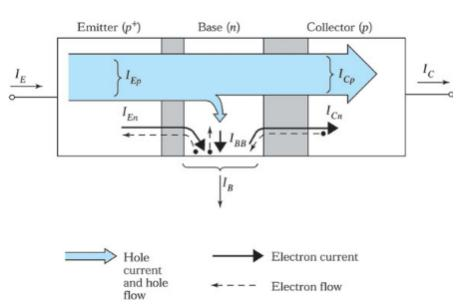
\includegraphics[width=11cm]{figures/ch01/bjt4.jpg}
\caption{Currents in active mode} 
\label{fig:bjt4}
\end{figure}

Nous caractérisons le transistor par le \emph{gain de courant en mode commun} $\alpha_0$, qui est le rapport entre $I_{Cp}$ et le courant d'émetteur :
$$
\alpha_0 \equiv \frac{I_{CP}}{I_E}
$$
Nous pouvons réécrire ceci comme :
$$
\alpha_0 = \frac{I_{Cp}}{I_{En} + I_{Ep}} = \Big(\frac{I_{Ep}}{I_{En} + I_{Ep}}\Big)  \Big(\frac{I_{Cp}}{I_{Ep}}\Big) = \alpha_T \; \gamma
$$
avec $\alpha_T$ le \emph{facteur de transfert de base} et $\gamma$ l'\emph{efficacité d'émetteur}. Pour un fonctionnement correct, nous exigeons que $I_{Ep} \gg I_{En}$, donc $\alpha_T \approx 1$. Cela peut être accompli en exigeant que le niveau de dopage de l'émetteur soit beaucoup plus élevé que celui de la base. Le facteur $\gamma$ peut être augmenté en diminuant la longueur de la base.\
Nous pouvons réécrire le courant de collecteur $I_C$ comme :
\begin{equation}
	\begin{split}
		I_C &= I_{Cp} + I_{Cn} = \alpha_T I_{Ep} = \alpha_0 I_E + I_{Cn} \\
		&= \alpha_0 I_E + I_{CB0}
	\end{split}
	\label{eq:bjt1}
\end{equation}
où $I_{CB0}$ est le courant de fuite entre le collecteur et la base avec la jonction émetteur-base ouverte. Cela exprime que le courant de collecteur est une fraction ($0 < \alpha_0 < 1$) du courant d'émetteur, plus un courant de fuite.

\subsection{Distribution de porteurs en mode actif}
Afin de calculer les différents courants, nous devons d'abord déterminer la distribution de porteurs dans chaque région. Nous supposerons ce qui suit :
\begin{enumerate}
	\item Dopage uniforme dans chaque région
	\item Pas de courant de dérive de trous dans la base
	\item Le courant de saturation du collecteur est négligeable
	\item Seulement une injection de faible niveau
	\item Pas de génération-recombinaison dans la zone de déplétion
	\item Pas de résistance série dans le dispositif
\end{enumerate}

Nous supposerons que $x=0$ correspond à la fin de la zone de déplétion émetteur-base, et $x=W$ au début de la zone de déplétion base-collecteur. À partir de l'équation de continuité pour les porteurs minoritaires dans la région de base:
$$
\frac{dp_n}{dt} = - \frac{(p_n-p_{n0})}{t_p} - \frac{1}{q} \frac{d J_p}{dx} + g \text{ avec }  J_p = q \mu_p p E + q D_p \frac{dp_n}{dx}
$$
Si nous supposons un état stationnaire, sans champ électrique et sans autres mécanismes de génération, l'équation se réduit à:
$$
D_p \frac{d^2 p_n}{dx^2} = \frac{(p_n-p_{n0})}{t_p}
$$
Cette équation a comme solution générale
$$
p_n(x) = p_{n0} + C_1  \; e^{x/L_p} + C_2 \;  e^{-x/L_p}
$$
avec $L_p = \sqrt{D_p t_p}$ la soi-disant \emph{longueur de diffusion} des trous dans le semi-conducteur de type n. Les constantes $C_1$ et $C_2$ peuvent être déterminées par les conditions aux limites:
\begin{itemize}
	\item $p_n(0) = p_{n0} ; e^{qV_{EB}/kT}$ car c'est la concentration standard à la limite de la région de déplétion, comme dans l'équation \ref{eq:density_junction} du chapitre \ref{ch:pnjunction},
	\item $p_n(W) = 0$ car tous les trous à $x=W$ seront balayés à travers la région de charge d'espace base-collecteur par le champ électrique induit.
\end{itemize}
La résolution pour $C_1$ et $C_2$ conduit à une distribution assez complexe. Cependant, si $W/L_p \ll 1$, nous pouvons simplifier et obtenir:
$$
p_n(x) = p_{n0}\; e^{qV_{EB}/kT} \; \Big(1 - \frac{x}{W} \Big)
$$
La concentration de porteurs minoritaires diminue donc linéairement dans la base. De manière similaire, nous pouvons trouver une expression pour les porteurs minoritaires (électrons) dans l'émetteur et le collecteur. Les résultats sont:
\begin{equation}
    \begin{split}
        n_E(x) &= n_{E0} + n_{E0} (e^{qV_{EB}/kT} - 1) e^{(x+x_E)/L_E}\\
        n_C(x) &= n_{C0} - n_{C0} e^{(x-x_C)/L_C}
    \end{split}
\end{equation}
Ces distributions sont également représentées dans la figure \ref{fig:bjt5}. Une fois que les concentrations de porteurs sont connues, les courants sont facilement calculés car ils sont proportionnels au gradient de concentration :
\begin{itemize}
    \item $I_{Ep} = A \Big(-q D_p \frac{dp_n}{dx}|_{x=0}\Big) = \frac{qAD_p \; p_{n0}}{W} e^{qV_{EB}/kT}$
    \item $I_{En} = A \Big(-q D_E \frac{dn_E}{dx}|_{x=-x_E}\Big) = \frac{qAD_E \; n_{E0}}{L_E} (e^{qV_{EB}/kT}-1)$
    \item \ldots
\end{itemize}
En combinant ces résultats, on obtient les expressions pour les trois courants terminaux :
\begin{itemize}
	\item $I_E = a_{11} (e^{qV_{EB}/kT} - 1) + a_{12}$
	\item $I_C = a_{12} (e^{qV_{EB}/kT} - 1) + a_{22}$
	\item $I_B = I_E - I_C$
\end{itemize}
où tous les $a_{ij}$ dépendent des caractéristiques du transistor comme les concentrations de dopage et les dimensions. 
\begin{figure}[h!]
\centering
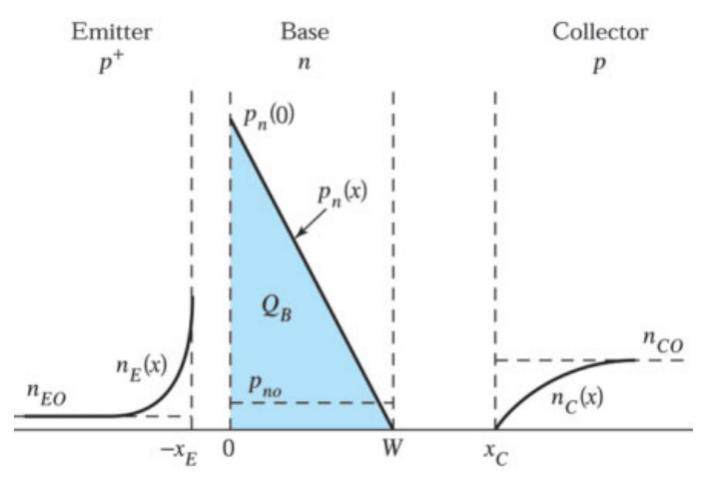
\includegraphics[width=10cm]{figures/ch01/bjt5.jpg}
\caption{Distribution de porteurs minoritaires en mode actif.} 
\label{fig:bjt5}
\end{figure}

\subsection{Modes de fonctionnement et équations d'Ebers-Moll}
\label{sec:modes_de_fonctionnement}
En fonction des signes de $V_{EB}$ et $V_{CB}$, nous pouvons distinguer $4$ modes de fonctionnement différents. Nous avons déjà étudié le cas où $V_{EB} > 0$ et $V_{CB} < 0$, à savoir le mode actif. Les autres modes sont représentés sur la figure \ref{fig:bjt_modes}, ainsi que la distribution des porteurs minoritaires dans l'émetteur, la base et le collecteur.
\begin{figure}[h!]
	\centering
	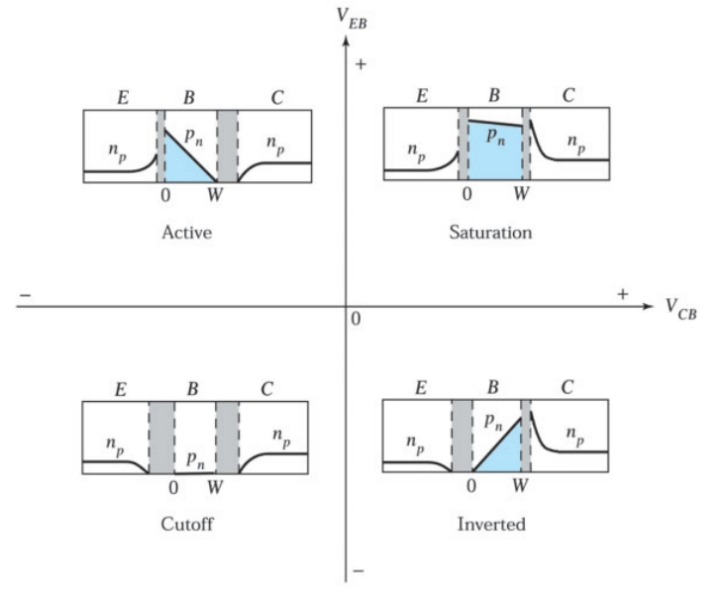
\includegraphics[width=12cm]{figures/ch01/bjt_modes.jpg}
	\caption{Modes de fonctionnement}
	\label{fig:bjt_modes}
\end{figure}
En mode saturation, les deux jonctions sont polarisées directement. La distribution de porteurs minoritaires à la limite de chaque région de déplétion n'est pas nulle, comme dans le mode actif. De faibles tensions de polarisation conduisent à un courant de sortie élevé. Le transistor agit comme un interrupteur fermé.\\
En mode coupure, les deux jonctions sont polarisées inversement. Seul un faible courant circulera. Le transistor est un interrupteur ouvert.\\
En mode inversé, l'émetteur et le collecteur sont inversés. Le comportement n'est cependant pas exactement comme dans le mode actif, car les niveaux de dopage dans l'émetteur et le collecteur sont différents.\\
Tous ces modes peuvent être analysés de manière similaire à ce que nous avons fait pour le mode actif. Cette analyse conduit aux \emph{équations d'Ebers-Moll} qui sont utilisées pour modéliser le BJT dans des simulateurs comme SPICE.\\
\textbf{TODO : Ajouter les équations d'Ebers-Moll et les circuits équivalents.}

\subsection{Configuration Émetteur Commun}
Jusqu'à présent, nous avons maintenu la base à une tension fixe. Cependant, l'utilisation la plus courante du transistor bipolaire est avec l'émetteur à une tension fixe comme dans la figure \ref{fig:bjt6}(a). Cette configuration a $V_{EB}$ et $I_B$ en entrée, et $I_C$ et $V_{EC}$ en sortie.\
Nous pouvons exprimer $I_C$ en fonction de $I_B$ en substituant $I_E = I_B + I_C$ dans l'équation \ref{eq:bjt1}:
$$
I_C = \alpha_0 (I_B + I_C) + I_{CBO}
$$
La résolution de l'équation \ref{eq:bjt1} pour $I_C$ donne:
\begin{equation}
    \begin{split}
        I_C &= \frac{\alpha_0}{1-\alpha_0} I_B + \frac{I_{CB0}}{1 - \alpha_0}\\
            &= \beta_0 I_B + I_{CE0}
        \label{eq:bjt2}
    \end{split}
\end{equation}
où $\beta_0 = \frac{\alpha_0}{1-\alpha_0}$ est le \emph{gain de courant commun-émetteur} et $I_{CE0} = \frac{I_{CB0}}{1-\alpha_0}$ est le courant de fuite collecteur-émetteur. Ce courant est toujours présent, même si $I_B = 0$, et rend le transistor bipolaire très mauvais comme interrupteur car il fuira du courant quand il est fermé.\\
Dans la configuration précédente, base commune, et avec $\alpha_0 \approx 1$, un changement du courant d'émetteur $I_E$ produit un changement d'environ la même quantité dans le courant de collecteur $I_C$ et un changement beaucoup plus petit dans le courant de base (facteur de $1-\alpha_0$). Pour obtenir une amplification de courant, le changement est initié dans le courant de base plutôt que dans le courant d'émetteur. Cela fait changer le courant de collecteur par un facteur de $\frac{\alpha_0}{1 - \alpha_0} = \beta_0$.\\
Lorsque $\alpha_0$ est proche de un, $\beta_0$ devient très grand. C'est une bonne chose car cela nous permet d'amplifier le courant de base $I_B$. Cependant, $\beta_0$ peut beaucoup varier d'un transistor à l'autre. C'est pourquoi nous explorerons des techniques de polarisation qui atténuent la variabilité de $\beta_0$.


\begin{figure}[h!]
\centering
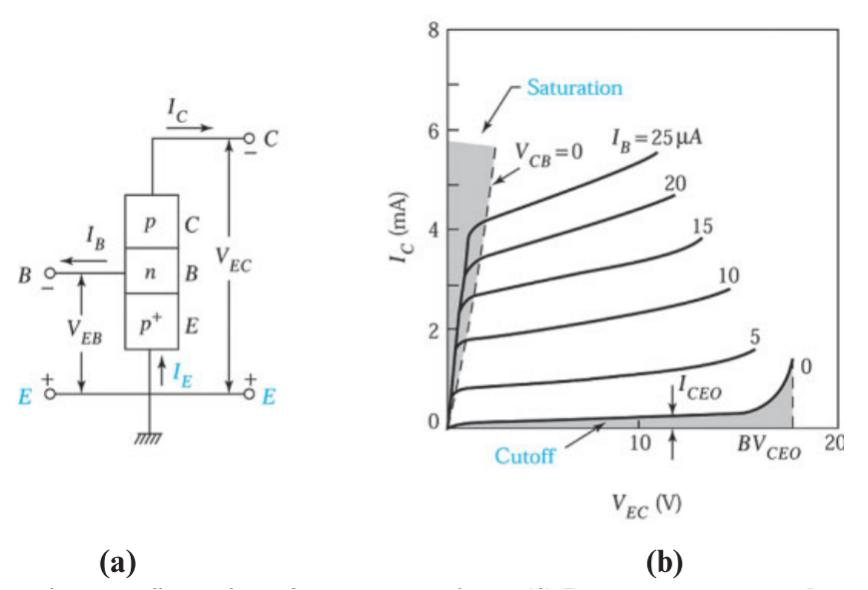
\includegraphics[width=10cm]{figures/ch01/bjt6.jpg}
\caption{BJT in common-emitter configuration (a) and I-V characteristic (b)} 
\label{fig:bjt6}
\end{figure}

La caractéristique I-V définissant une configuration émetteur commun est montrée dans la figure \ref{fig:bjt6}(b). Si $V_{EC}$ est trop faible, $V_{CB}$ est positif et la jonction base-collecteur n'est pas polarisée en inverse. Le transistor est en mode saturation. Ainsi, $V_{EC}$ doit être supérieur à un certain seuil pour mettre le transistor en mode actif. Cette valeur est appelée $V_{EC, Sat}$ et est d'environ $0,2$ V.\
Lorsque $V_{EC} > V_{EC, Sat}$, nous pouvons dire, sur la base de l'équation \ref{eq:bjt2}, que $I_C \approx \beta_0 I_B$ et donc indépendant de $V_{EC}$. C'est un comportement idéal, car nous contrôlons maintenant le courant de sortie $I_C$ avec le courant d'entrée $I_B$ et non avec la tension de sortie $V_{EB}$. Cependant, comme on peut le voir sur la figure, les caractéristiques I-V ne sont pas entièrement plates et dépendent donc encore de $V_{EB}$. Cela est dû à l'effet Early et sera abordé dans la prochaine section.\
Si $V_{EB}$ est inférieur à $0,6$ V, la jonction émetteur-base n'est pas polarisée en direct et $I_B$ est très faible. On dit que le transistor est en coupure. Le seul courant qui continue de circuler de l'émetteur vers le collecteur est le courant de fuite $I_{CE0}$.

\subsection{Effet Early}
En principe, $I_C$ devrait être indépendant de la tension de la jonction base-collecteur $V_{BC}$. Cependant, lorsque $V_{BC}$ augmente, la largeur de la région de charge d'espace entre la base et le collecteur augmente, comme prédit par l'équation \ref{eq:SCR_width_bias} où $V_F = -V_{BC}$. Cela signifie que la longueur effective de la base diminue et cela a deux effets :
\begin{enumerate}
	\item Plus de trous provenant de l'émetteur atteindront le collecteur car il y a moins de place pour la recombinaison. Effectivement, le facteur de transfert de base $\alpha_T$ augmente.
	\item Le courant de trou est déterminé par la pente de la concentration de trous dans la base, comme vu précédemment. Lorsque $W$ diminue, tout en maintenant les conditions aux limites, le courant de diffusion de trou $I_{Ep}$ augmente. L'augmentation de la pente (en termes absolus) est montrée dans la figure \ref{fig:bjt7}(a).
\end{enumerate}

Les deux effets contribuent à une augmentation de $I_C$ lorsque $V_{CB}$ (ou $V_{EC}$ en configuration émetteur commun) augmente et que $I_B$ reste constant. Ce phénomène est appelé l'\emph{effet Early}. Nous pouvons montrer que toutes ces courbes de courant non plates dans la caractéristique I-V (voir figure \ref{fig:bjt7}(b)) passent par le même point sur l'axe V lorsqu'elles sont étendues. La tension correspondante est la tension Early $V_A$.

\begin{figure}[h!]
\centering
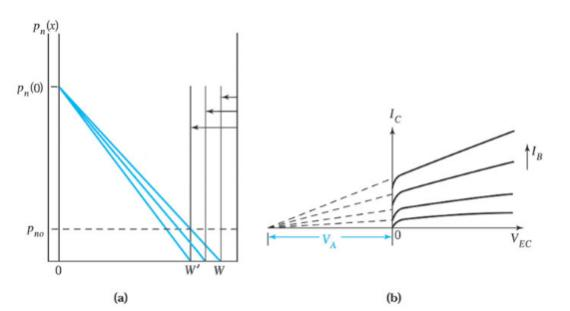
\includegraphics[width=10cm]{figures/ch01/bjt7.jpg}
\caption{Schematic diagram of (a) the Early effect and (b) Early voltage $V_A$} 
\label{fig:bjt7}
\end{figure}

%\section{Field-Effect Transistor}
%\newpage
%\section{JFET}
%PM

\newpage
\section{MOSFET}
\label{sec:mosfet}
Le transistor à effet de champ métal-oxyde-semi-conducteur, ou \emph{MOSFET}, est un transistor basé sur l'effet de champ. Il possède une grille isolée, constituée d'un conducteur tel que du métal ou du poly-silicium. Cette borne est isolée du reste du dispositif par une fine couche de $SiO_2$ qui sert de diélectrique. La tension appliquée à la grille détermine la conductivité du dispositif et peut donc contrôler le courant entre les deux autres bornes nommées source et drain. Cette capacité à modifier la conductivité en fonction de la tension appliquée peut être utilisée pour amplifier ou commuter des signaux électroniques. La Figure \ref{fig:mosfet1}(a) montre la structure d'un MOSFET, tandis que la Figure \ref{fig:mosfet1}(c) montre ses symboles ainsi que les trois bornes.
\subsection{Description et fonctionnement}
La Figure \ref{fig:mosfet1}(b) montre la section transversale d'un MOSFET à canal n. La source (S) et le drain (D) sont tous deux des contacts $n^+$ et sont isolés l'un de l'autre par le substrat de type p. Lorsque la tension sur la grille augmente, les trous dans le matériau de type p sont expulsés et la région sous la grille devient appauvrie en porteurs de charge. Si la tension de la grille augmente encore plus, les électrons présents dans le volume de type p en tant que porteurs minoritaires sont attirés vers la région sous la grille. Une couche étroite d'électrons entre la source et le drain est formée et la conduction d'électrons entre la source et le drain devient possible. Si la densité électronique sous la grille est égale à la concentration en trous dans le volume, une inversion s'est produite et nous disons qu'un canal s'est formé. La tension de la grille à laquelle cette inversion de type p à type n se produit est appelée tension seuil $V_T$.\
Pour qu'un courant s'écoule de la source au drain, nous avons besoin non seulement d'un canal, mais également d'une différence de tension positive entre le drain et la source. À mesure que nous augmentons la tension au niveau du drain, le courant augmente, mais en même temps, la profondeur du canal au niveau du drain diminue car $V_{GD} < V_{GS}$. À un certain moment, la différence de tension entre la grille et le drain n'est plus suffisante pour maintenir un canal de type n ($V_{GD} = V_T$). Nous appelons cela \emph{pinch-off} et disons que le transistor est saturé. Le courant entre le drain et la source n'augmente plus à mesure que la tension de drain augmente mais reste constant.

\begin{figure}[h!]
\centering
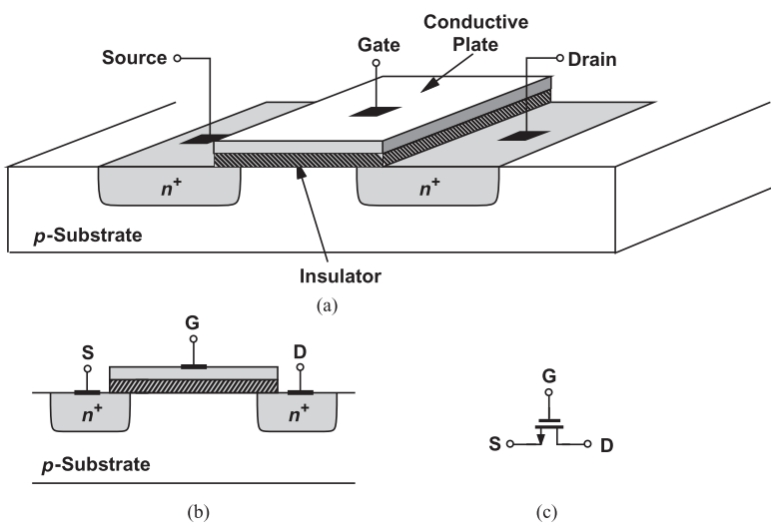
\includegraphics[width=10cm]{figures/ch01/mosfet1b.jpg}
\caption{Schematic diagram of a n-channel MOSFET: (a) structure, (b) side view, (c) symbol} 
\label{fig:mosfet1}
\end{figure}

Les dimensions d'un MOSFET peuvent devenir très petites ; l'épaisseur typique de l'oxyde de grille $t_{ox}$ est d'environ $15 \AA$ et diminue avec chaque nouvelle génération. La longueur du canal $L$ est généralement de plusieurs dizaines de nanomètres.

\subsection{Condensateur MOS}
La région sous la grille est appelée un condensateur MOS. Dans les circuits intégrés, il peut stocker des charges et constitue la base de construction pour les dispositifs à transfert de charges (CCD). Un MOSFET peut donc être considéré comme un condensateur MOS et deux jonctions pn placées immédiatement adjacentes. Nous verrons brièvement comment la charge s'accumule dans le semi-conducteur lorsqu'une tension est appliquée à la grille métallique.\
La figure \ref{fig:moscap} représente un condensateur MOS avec la grille à gauche et le semi-conducteur de type p à droite de l'oxyde. Si une tension négative $V < 0$ est appliquée à la plaque métallique de la grille, comme dans \ref{fig:moscap}(a), les porteurs positifs sont attirés vers l'interface $SiO_2 - Si$. Aucun courant ne circule dans le dispositif, donc le niveau de Fermi reste constant. La distribution des porteurs dépend de la différence $E_i - E_F$: $p_p = n_i e^{(E_i - E_F)/kT}$, donc les bandes de conduction et de valence à l'interface doivent se courber vers le haut pour augmenter $E_i - E_F$ car $E_F$ est constant. Les trous "flottent" vers le maximum dans la bande de valence et s'accumulent à l'interface.\
Si $V > 0$, comme dans \ref{fig:moscap}(b), les trous sont repoussés de l'interface et les bandes se courbent vers le haut. Au départ, tous les donneurs accepteurs sont exposés et une couche de charge de profondeur $W$ est créée à l'intérieur du semi-conducteur. La densité de charge induite par unité de surface est $Q_d = q N_A W$. Nous appelons ce processus \emph{déplétion}. Si $V$ augmente encore et que les bandes se courbent encore plus, le niveau de Fermi intrinsèque tombera en dessous du niveau de Fermi réel comme dans \ref{fig:moscap}(c) et les électrons afflueront vers l'interface car l'exposant dans l'expression $n_p = n_i e^{(E_F - E_i)/kT}$ devient positif. Ce processus est appelé \emph{inversion} et est la condition nécessaire pour former un canal dans un MOSFET. Le canal est une région très chargée juste à droite de l'interface (voir la distribution de charge), séparée du semi-conducteur de type p par une région de déplétion relativement large. La tension où les niveaux de Fermi se croisent est la tension de seuil $V_T$ et nous désignons la charge associée $Q_n$.

\begin{figure}[h!]
\centering
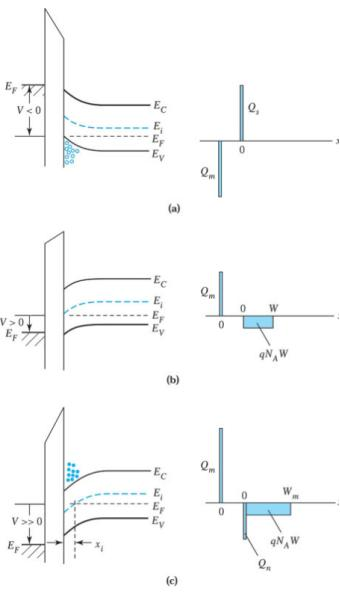
\includegraphics[width=7cm]{figures/ch01/moscap.jpg}
\caption{Band diagrams and charge distribution of a MOS capacitor in (a) accumulation, (b) depletion, and (c) inversion} 
\label{fig:moscap}
\end{figure}

\subsection{Caractéristique I-V}
\label{sec:MOS_IV}
Si $V$ est la différence de tension appliquée aux plaques d'un condensateur et $C$ la capacitance, alors la charge induite est $Q = CV$. Dans le cas du MOSFET de la figure \ref{fig:mosfet1}(b), nous ne nous intéressons qu'aux charges mobiles sous la grille, c'est-à-dire les électrons $Q_n$ attirés vers l'interface de la figure \ref{fig:moscap}(c), et non à la charge de déplétion $Q_d=qN_AW$. Cela signifie que $V=V_{GS}-V_T$ car aucune charge mobile n'existe pour $V_{GS}<V_T$ \footnote{Cette hypothèse sera révisée dans la section \ref{sec:subthreshold_conduction}}. Si nous supposons que le condensateur MOS a une capacité de grille $C_{ox}$ par unité de surface, cette relation devient
$$Q_n = W C_{ox} (V_{GS} - V_T)$$
avec $W$ la largeur du transistor. Notez que $Q_n$ est une densité de charge par unité de longueur. Comme la tension de drain et de source n'est pas la même, la tension de canal varie le long de la longueur du canal. Si nous désignons le potentiel de canal par $V(x)$, nous pouvons réécrire l'équation ci-dessus comme suit:
$$Q_n(x) = W C_{ox} (V_{GS} - V(x) - V_T)$$
où $V(x)$ va de zéro à $V_D$ si le canal n'est pas étranglé (figure \ref{fig:mosfet2}(a)).\\
Nous savons que le courant est la densité de charge multipliée par la vitesse des charges: $I_D=Q_n(x)\cdot v$. Le courant est un courant de dérive car nous appliquons un champ électrique $\mathcal{E}$ à travers le canal. Ainsi :
$$v = -\mu_n \mathcal{E} = \mu_n \frac{dV}{dx}$$
avec $\mu_n$ la mobilité des électrons. En substituant cela dans l'expression de $I_D$, nous trouvons :
$$I_D = W C_{ox} (V_{GS} - V(x) - V_T) \mu_n \frac{dV(x)}{dx}$$
En multipliant les deux côtés par $dx$ et en intégrant de $x = 0$ à la longueur de canal $L$ :
$$
 \int_{x=0}^{x=L} I_D dx = \int_{V(x)=0}^{V(x)=V_{DS}} \mu_n C_{ox} W (V_{GS}-V(x)-V_T)dV 
$$
Parce que $I_D$ est constant le long du canal, nous pouvons résoudre les deux intégrales et exprimer $I_D$ comme
\begin{equation}
\begin{split}
    I_D = \frac{1}{2} \mu_n C_{ox} \frac{W}{L} [ 2(V_{GS} - V_T) V_{DS} - V_{DS}^2 ]
\end{split}
\end{equation}
Ceci est une fonction parabolique qui atteint un maximum pour $V_{DS} = V_{GS} - V_T$ :
$$I_{D, max} = \frac{1}{2} \mu_n C_{ox} \frac{W}{L} (V_{GS} - V_T)^2$$
Nous avons déjà établi que la condition de saturation est $V_{GD} = V_T$ : à partir de ce point, le courant ne va plus augmenter lorsque $V_{DS}$ augmente car un effet de pincement s'est produit au drain. Étant donné que $V_{DG} = V_{DS} - V_{GS}$ et que lorsqu'un effet de pincement se produit $V_{DG} = -V_T$, nous pouvons réécrire cette condition sous la forme $V_{DS} = V_{GS} - V_T$, c'est-à-dire que le transistor est en saturation au maximum de la courbe. C'est la situation représentée dans la figure \ref{fig:mosfet2}(b) et (c). Lorsque $V_{DS}$ augmente, le point de pincement $P$ se rapproche de la source. La différence de potentiel dans le canal rétrécissant en $P$ reste à $V_{GS} - V_T$. Le transistor est en saturation\footnote{Notez que la saturation pour un MOSFET n'est pas le même concept que la saturation pour un BJT} et le courant de drain est - dans une première approximation - égal à :
\begin{equation}
    I_{D} = \frac{1}{2} \mu_n C_{ox} \frac{W}{L} (V_{GS} - V_T)^2
    \label{eq:sat_current}
\end{equation}
Notez que contrairement au BJT, il n'y a pas de courant continu à travers la grille.\footnote{Note sur la notation : nous utiliserons souvent $K$ pour le produit $\mu_n C_{ox}$.}

\begin{figure}[h!]
\centering
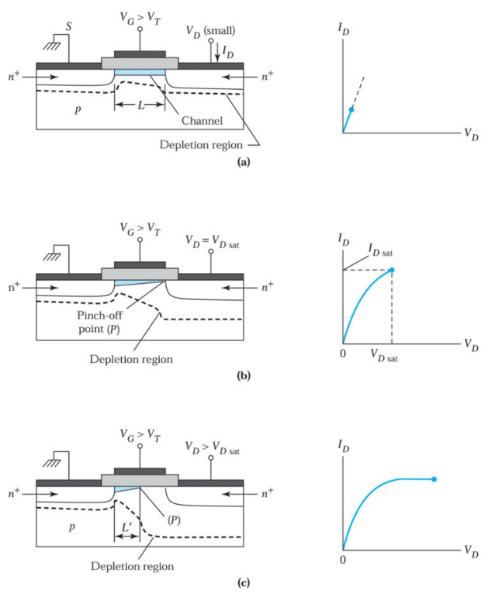
\includegraphics[width=12cm]{figures/ch01/mosfet2.jpg}
\caption{Operations of the MOSFET and output I-V characteristics. (a) Low drain voltage. (b) Onset of saturation. (c) Beyond saturation.} 
\label{fig:mosfet2}
\end{figure}

Si $V_{DS}$ est relativement petit, nous pouvons approximer $I_D$ comme suit :
$$I_D \approx  \mu_n C_{ox} \frac{W}{L} (V_{GS} - V_T) V_{DS}$$
Ceci est l'expression d'une résistance avec une valeur:
$$R_{on} = \frac{1}{\mu_n C_{ox} \frac{W}{L} (V_{GS} - V_T)}$$
Nous disons que le transistor est dans la région \emph{linéaire} ou \emph{triode}. Comme la résistance est une fonction de $V_{GS}$, le MOSFET dans cette région peut être considéré comme une résistance programmable.
%$$I_{D} = \frac{1}{2} \mu_n C_{ox} \frac{W}{L} (V_{GS} - V_T)^2$$

La figure \ref{fig:mosfet3} donne la caractéristique de sortie globale d'un MOSFET à canal N. Remarquez comment le point de transition de linéaire à saturation dépend de $V_{GS}$ : pour que le transistor soit en saturation, $V_{DS}$ doit être plus grand que la \emph{tension de suralimentation} $V_{ov} = V_{GS} - V_T$, également appelée tension de saturation $V_{DS, Sat}$. Ce n'est pas le cas pour le BJT, où nous avons utilisé une coupure fixe $V_{CE,sat}$ avec une valeur de $0,2$ V.

\begin{figure}[h!]
\centering
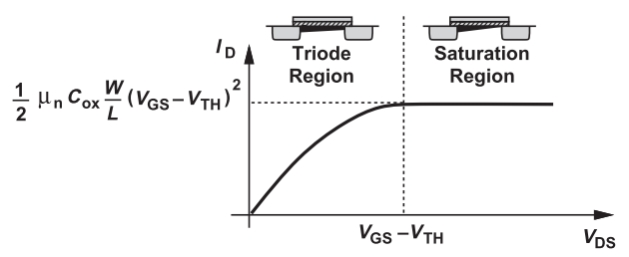
\includegraphics[width=10cm]{figures/ch01/mosfet3.jpg}
\caption{Overall MOSFET $I_D - V_{DS}$ characteristic} 
\label{fig:mosfet3}
\end{figure}
Nous avons étudié le MOSFET à canal N ou \emph{NMOS}. L'étude du MOSFET à canal P ou \emph{PMOS} est laissée en exercice pour le lecteur.

\subsection{Effets de Second Ordre}
Nous discuterons de plusieurs effets de second ordre qui feront que le MOSFET se comportera différemment du comportement idéal de la figure \ref{fig:mosfet3}.
\subsubsection{Modulation de la longueur du canal}
Remarquez que dans la figure \ref{fig:mosfet3}(c), la longueur effective du canal diminue à mesure que la tension de drain augmente (le point d'étranglement se déplace vers la gauche). Nous avons établi l'équation \ref{eq:sat_current} avec l'hypothèse implicite que $L$ est constant. Cependant, si la longueur effective du canal diminue, le courant $I_D$ augmentera avec l'augmentation de $V_{DS}$ et la caractéristique I-V de la figure \ref{fig:mosfet3} ne sera pas plate. Ceci est similaire à l'effet Early dans le BJT.\
Pour modéliser cela, nous supposons que $L$ ne change pas, mais incluons une dépendance explicite de $V_{DS}$ dans l'équation \ref{eq:sat_current} :
\begin{equation}
    I_{D} = \frac{1}{2} \mu_n C_{ox} \frac{W}{L} (V_{GS} - V_T)^2 \; (1 + \lambda V_{DS})
    \label{eq:sat_current2}
\end{equation}
Le facteur $\lambda$ est le \emph{coefficient de modulation de longueur de canal}. Pour diminuer $\lambda$, le concepteur peut augmenter la longueur du transistor, car cela rend l'impact relatif d'un changement de $L$ plus petit.
\subsubsection{Effet de corps}
Jusqu'à présent, nous avons supposé que le substrat de type p et la source de type n étaient connectés à une masse commune. Ce n'est cependant pas toujours le cas dans les circuits réels, où la source peut être connectée à des tensions supérieures à celles du substrat. Même dans ce cas, la jonction pn entre la source et le substrat est toujours polarisée en inverse et le dispositif fonctionne correctement.\\
Cependant, quelque chose change lorsque la tension de la source augmente par rapport au substrat: lorsque la source devient plus positive par rapport au substrat, la tension de seuil $V_T$ augmente. Appelé "effet de corps", ce phénomène est formulé comme
$$V_T = V_{T0} + \gamma (|2\phi_F + V_{SB} - |2\phi_F|)$$
où $V_{SB}$ est la différence de tension entre la source et le substrat (bulk), $V_{T0}$ est la tension de seuil lorsque $V_{SB} = 0$ et $\gamma$ et $\phi_F$ sont des paramètres dépendants de la technologie.
\subsubsection{Conduction sub seuil}
\label{sec:subthreshold_conduction}
Nous avons supposé que le MOSFET s'allume brusquement lorsque la tension de la grille dépasse la tension de seuil. En pratique cependant, le dispositif s'allume progressivement et il y a déjà un courant source-drain avant que $V_T$ soit atteint. Ce courant dépend exponentiellement de $V_{GS}$, de manière similaire à un BJT. Appelé la \emph{conduction sub seuil}, cet effet est devenu un problème critique dans les dispositifs MOS modernes.